\documentclass[../basicOrbitalDynamics.tex]{subfiles}
\graphicspath{{\subfix{../images/}}}
\begin{document}

\bigskip\bigskip
\subsection{Kepler's First Law}\label{sec:Kepler's First Law}

Kepler's first law states that all orbits are conic sections. A conic section, when graphed in cartesian coordinates, follows
\[\left(\frac{x\pm{}c}{a}\right)^2+\left(\frac{y}{b}\right)^2=1\]

Where $a$ is the semi-major axis, $b$ is the semi-minor axis, and $c$ is the distance from the origin to the center of the ellipse. Note the $\pm$ is to accommodate an ellipse with either focus on the origin.

The orbit equation with the semi-latus rectum (Equation~\eqref{Polar with p, e}) will be used, as it is slightly more concise than Equation \eqref{Polar Final}. $\omega$ will be set to zero, as it does not dictate the shape of the orbit. For the sake of conversion between polar and cartesian coordinates, the inclination of the orbit will be assumed to be zero ($\hat{u}_n=\hat{z}$). Note that this algebra is somewhat tedious. If there is any section in which the ``throw it into Desmos and see if it lines up'' approach to math should be taken, this is the section.
\begin{align*}
    r                                                                                          & =\frac{p}{1+e\cos(\theta)}                                      \\
    r(1+e\cos(\theta))                                                                         & = p                                                             \\
    r                                                                                          & =p-er\cos(\theta)                                               \\
    r^2                                                                                        & =(p-er\cos(\theta))^2                                           \\
    x^2+y^2                                                                                    & =(p-ex)^2                                                       \\
    x^2+y^2                                                                                    & =e^2x^2-2epx+p^2                                                \\
    x^2-e^2x^2+2epx-p^2                                                                        & =-y^2                                                           \\
    (1-e^2)x^2+2epx-p^2                                                                        & =-y^2                                                           \\
    \left(\sqrt{1-e^2}x+\frac{ep}{\sqrt{1-e^2}}\right)^2-\left(\frac{p}{\sqrt{1-e^2}}\right)^2 & =-y^2                                                           \\
    \left(x+\frac{ep}{1-e^2}\right)^2-\left(\frac{p}{1-e^2}\right)^2                           & =-\left(\frac{y}{\sqrt{1-e^2}}\right)^2                         \\
    \left(\frac{x+\frac{ep}{1-e^2}}{\frac{p}{1-e^2}}\right)^2-1                                & =-\left(\frac{\frac{y}{\sqrt{1-e^2}}}{\frac{p}{1-e^2}}\right)^2 \\
    \left(\frac{x(1-e^2)}{p}+e\right)^2-1                                                      & =-\left(\frac{y\sqrt{1-e^2}}{p}\right)^2                        \\
    \left(\frac{x(1-e^2)}{p}+e\right)^2+\left(\frac{y\sqrt{1-e^2}}{p}\right)^2                 & =1                                                              \\
    \left(\frac{x(1-e^2)}{a(1-e^2)}+e\right)^2+\left(\frac{y\sqrt{1-e^2}}{a(1-e^2)}\right)^2   & =1                                                              \\
    \left(\frac{x}{a}+e\right)^2+\left(\frac{y}{a\sqrt{1-e^2}}\right)^2                        & =1                                                              \\
\end{align*}

\begin{equation}\label{Orbit Cartesian}
    \left(\frac{x+ea}{a}\right)^2+\left(\frac{y}{a\sqrt{1-e^2}}\right)^2=1
\end{equation}

This is in the form of
\[\left(\frac{x+c}{a}\right)^2+\left(\frac{y}{b}\right)^2=1\]

The $+$ denotes that the right focus (as opposed to the left one) is at the origin. It was already known that $a$ was the semi-major axis, however this equation also yields some other useful information. This formula implies that the semi-minor axis $b=a\sqrt{1-e^2}$, and that the distance from the origin (which is at the focus of the ellipse) to its center is $c=ea$.

This equation is also valid for hyperbolic orbits, as $a\sqrt{1-e^2}$ will be purely complex, but then will be squared to become negative. For parabolic orbits, however, this equation is not valid. A similar approach is valid for hyperbolic orbits in which $e=1$.

\begin{align*}
    r                 & =\frac{p}{1+e\cos(\theta)}              \\
    r                 & =\frac{p}{1+\cos(\theta)}               \\
    r(1+\cos(\theta)) & = p                                     \\
    r+r\cos(\theta)   & = p                                     \\
    r                 & = p-r\cos(\theta)                       \\
    r^2               & = p^2-2pr\cos(\theta)+(r\cos(\theta))^2 \\
    x^2+y^2           & = p^2-2px+x^2                           \\
    y^2               & = p^2-2px                               \\
\end{align*}

Notice that the multiplicity of $y$ is 2, and the multiplicity of $x$ is 1. This is a parabola that opens up in the $-x$ direction.

\bigskip\bigskip
\subsection{Kepler's Second Law}\label{sec:Kepler's Second Law}

Kepler's second law states that the line connecting an orbiting body and the body it orbits sweeps out equal area in equal quantities of time.
\begin{figure}[H]
    \centering
    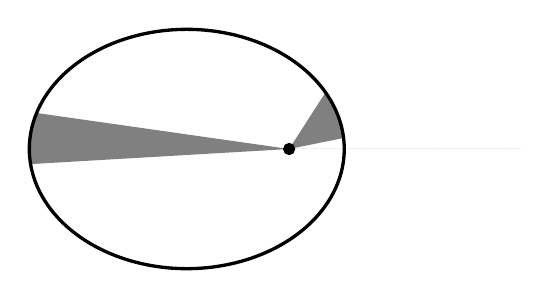
\begin{tikzpicture}[>=latex]
        \def\ecc{0.65}
        \def\SMA{2}
        \def\ap{\fpeval{\SMA*(1+\ecc)}}
        \def\pe{\fpeval{\SMA*(1-\ecc)}}
        \def\slr{\fpeval{\SMA*(1-\ecc^2)}}
        \def\thta{3}
        \def\thtb{0.2}
        \def\arca{0.2}
        \def\arcb{0.8}


        \fill[fill=gray] (0,0) -- ++(\thta:{3*cos(\thta r)}) plot[domain=\thta:\thta+\arca] (xy polar cs:angle=\x r,radius= {(\slr)/(1+\ecc*cos(\x r))})--(0,0)--cycle;
        \fill[fill=gray] (0,0) -- ++(\thtb:{3*cos(\thtb r)}) plot[domain=\thtb:\thtb+\arcb] (xy polar cs:angle=\x r,radius= {(\slr)/(1+\ecc*cos(\x r))})--(0,0)--cycle;

        \draw[domain=0:2*pi,samples=500, very thick] plot ({deg(\x)}:{(\slr)/(1+\ecc*cos(\x r))});

        \filldraw[] (0,0) circle (2pt);
    \end{tikzpicture}

    \caption{An orbit with multiple areas shaded, each of which is swept out in equal time}
\end{figure}

To prove this law, the area will be found of a segment of the ellipse tranversed from $t_1$ to $t_2$.
\begin{align*}
    \text{Area} & =\iint{}dA                                               \\
                & = \int_{\theta(t_1)}^{\theta(t_2)}\int_{0}^{r}rdrd\theta \\
                & = \int_{\theta(t_1)}^{\theta(t_2)}\frac{1}{2}r^2d\theta  \\
                & = \int_{t_1}^{t_2}\frac{1}{2}r^2\frac{d\theta}{dt}dt     \\
                & = \int_{t_1}^{t_2}\frac{1}{2}r^2\dot{\theta}dt           \\
\end{align*}

Recall from Equation \eqref{Angular Momentum:h unknown} that $h=r^2\dot{\theta}$.
\begin{align*}
    \text{Area} & = \int_{t_1}^{t_2}\frac{1}{2}r^2\dot{\theta}dt \\
                & = \int_{t_1}^{t_2}\frac{1}{2}hdt               \\
                & = \frac{h}{2}\int_{t_1}^{t_2}dt                \\
                & = \frac{h}{2}\Delta{}t                         \\
\end{align*}

This expression is expression is independent of where in the orbit a satellite is.
\begin{equation}\label{Kepler's First Law}
    \text{Area Traversed} = \frac{h}{2}\Delta{}t
\end{equation}

\bigskip\bigskip
\subsection{Conservation of Specific Energy}\label{sec:Conservation of Energy}

Specific energy $\varepsilon$ is, like angular momentum, conserved. It is defined as the sum of specific kinetic and specific potential energy.
\begin{align*}
    \varepsilon & =\frac{\text{KE}+\text{PE}}{m}                             \\
                & =\frac{1}{m}(\text{KE}+\text{PE})                          \\
                & =\frac{1}{m}\left(\frac{1}{2}mv^2+\frac{-\mu{}m}{r}\right) \\
\end{align*}
\begin{equation}\label{Specific Energy Physical}
    \varepsilon=\frac{v^2}{2}-\frac{\mu{}}{r}
\end{equation}

Conservation of energy can be proven quite simply with physical reasoning, as there is no external force (external to the system, with said system comprising of the orbited body and the orbiting body) to do work. With no external work done, there is no source of energy change. However, it can now be shown that specific energy is conserved through differentiation with respect to distance travelled. Recall that $a_r=\frac{-\mu}{r^2}$ (Equation \eqref{Differential Equation:r}) and $a_\theta=0$ (Equation \eqref{Differential Equation:theta}) from Section \ref{sec:Differential Equation Setup}.
\begin{align*}
    \frac{d\varepsilon}{ds} & =\frac{d}{ds}\left(\frac{|v|^2}{2}\right)-\frac{d}{ds}\left(\frac{\mu}{|r|}\right) \\
                            & =|v|\frac{d|v|}{ds}+\frac{\mu{}}{|r|^2}\frac{d|r|}{ds}                             \\
                            & =|v|\frac{d|v|}{dt}\frac{dt}{ds}+\frac{\mu{}}{|r|^2}\frac{d|r|}{dt}\frac{dt}{ds}   \\
                            & =\frac{dt}{ds}\left(|v|\frac{d|v|}{dt}+\frac{\mu{}}{|r|^2}\frac{d|r|}{dt}\right)   \\
                            & =\frac{dt}{ds}\left(|v|a_\parallel-a_r\frac{d|r|}{dt}\right)                       \\
                            & =\frac{dt}{ds}(|v|(\vv{a}\cdot\hat{v})-a_rv_r)                                     \\
                            & =\frac{dt}{ds}(\vv{a}\cdot\vv{v}-a_rv_r)                                           \\
                            & =\frac{dt}{ds}((a_rv_r+a_\theta{}v_\theta)-a_rv_r)                                 \\
                            & =\frac{dt}{ds}(a_\theta{}v_\theta)                                                 \\
                            & =\frac{dt}{ds}(0v_\theta)                                                          \\
                            & =0                                                                                 \\
\end{align*}

Because the derivative of $\varepsilon$ with respect to distance travelled is zero, it does not change across an orbit and will be conserved.
\end{document}